\newcommand{\Feat}{\text{Feat}}
\newcommand{\Exp}{\text{Exp}}
\captionsetup[table]{skip=2pt}


\section{Introduction} \label{sec:Introduction}
% A few sentences placing the work in high-level context. Limit it to a few paragraphs at most; your report is on reproducing a piece of work, you don’t have to motivate that work.
Recent research has revealed that visual models like convolutional neural networks (CNNs) can exhibit societal biases based on protected characteristics such as race, gender, and age \cite{buolamwini2018gender, das2018mitigating, kortylewski2018empirically, wang2020mitigating, hendricks2018women}.
Transparency and interpretability of these models are crucial because it helps us make sense of their decision-making processes while identifying implicit biases that may negatively affect the fairness of their predictions.
\\\\
In order to improve this aspect of deep neural networks, Yang et al. introduce the framework \textit{Latent Visual-Semantic Filter Attention} (LaViSE) \cite{yang2022explaining}, which aims to generate textual explanations about the decision-making process of any CNN.
\\\\
This report aims to replicate the authors' findings, verify their results and perform additional experiments to provide insights into the generalizability of their approach. Our main contributions comprise the following:
\begin{enumerate}
    \item Enhancing the original code's completeness, reproducibility, maintainability, and efficiency (see section \ref{sec:Improving the codebase}).
    \item Replicating the authors' key experiments to assess their results' reproducibility and evaluate the resources required for replication, including computational cost, development effort, and communication with the authors (see sections \ref{sec:Pre-processing}, \ref{sec:Hyperparameters}, \ref{sec:Computational requirements}, \ref{sec:Results reproducing original paper} and \ref{sec:Discussion}).
    \item Extending and evaluating the experiments to verify the authors' claim of their method being generalizable across different CNNs (see section \ref{sec:Results beyond original paper}).
\end{enumerate}
For further reproducibility, we have made all the code that produced the results in this report publicly available\footnote{\url{https://github.com/ErikBuis/FACT2023}}.


\section{Scope of reproducibility} \label{sec:Scope of reproducibility}
% In this section, you should mitivate what you do and why. if you claim something, at least give a refeernce to where in the report you will motivate it more!
Existing global post-hoc approaches vary in their model explanation method (whether CNNs are explained semantically or visually) and their focus (whether individual filters or the model as a whole is interpreted). However, they tend to rely upon needing access to the original training dataset and may have limited generalizability to other models \cite{park2018multimodal}. The original paper tries to overcome these limitations by proposing a framework that uses a separate dataset to train a separate model, which in turn generates semantic explanations of the filters of the model we want to interpret. This approach is post-hoc, because we can see existing models that we want to interpret as ``black boxes'' that do not have to be retrained.
\\\\
This reproducibility analysis will verify the main claims made by the authors, which are:
\begin{enumerate}
    \item The proposed framework creates an accurate mapping between the visual and semantic space by using generic object detection datasets.
    \item The proposed framework can generate novel descriptions for learned filters beyond the categories defined in the reference dataset.
    \item The proposed framework can analyze any trained CNN, regardless of whether or not the original training data is available.
\end{enumerate}

The remainder of this study is organized as follows. Firstly, section \ref{sec:Latent Visual-Semantic Filter Attention} provides background information about the framework proposed. Next, we present our approach to reproduce this work in section \ref{sec:Methodology}. Section \ref{sec:Results} summarizes our results and compares them to the original paper. Finally, section \ref{sec:Discussion} evaluates the ease and difficulty of reproducing the results, discussing which aspects were more straightforward and which posed challenges.


\section{Latent Visual-Semantic Filter Attention} \label{sec:Latent Visual-Semantic Filter Attention}
\begin{figure}[b!]
    \centering
    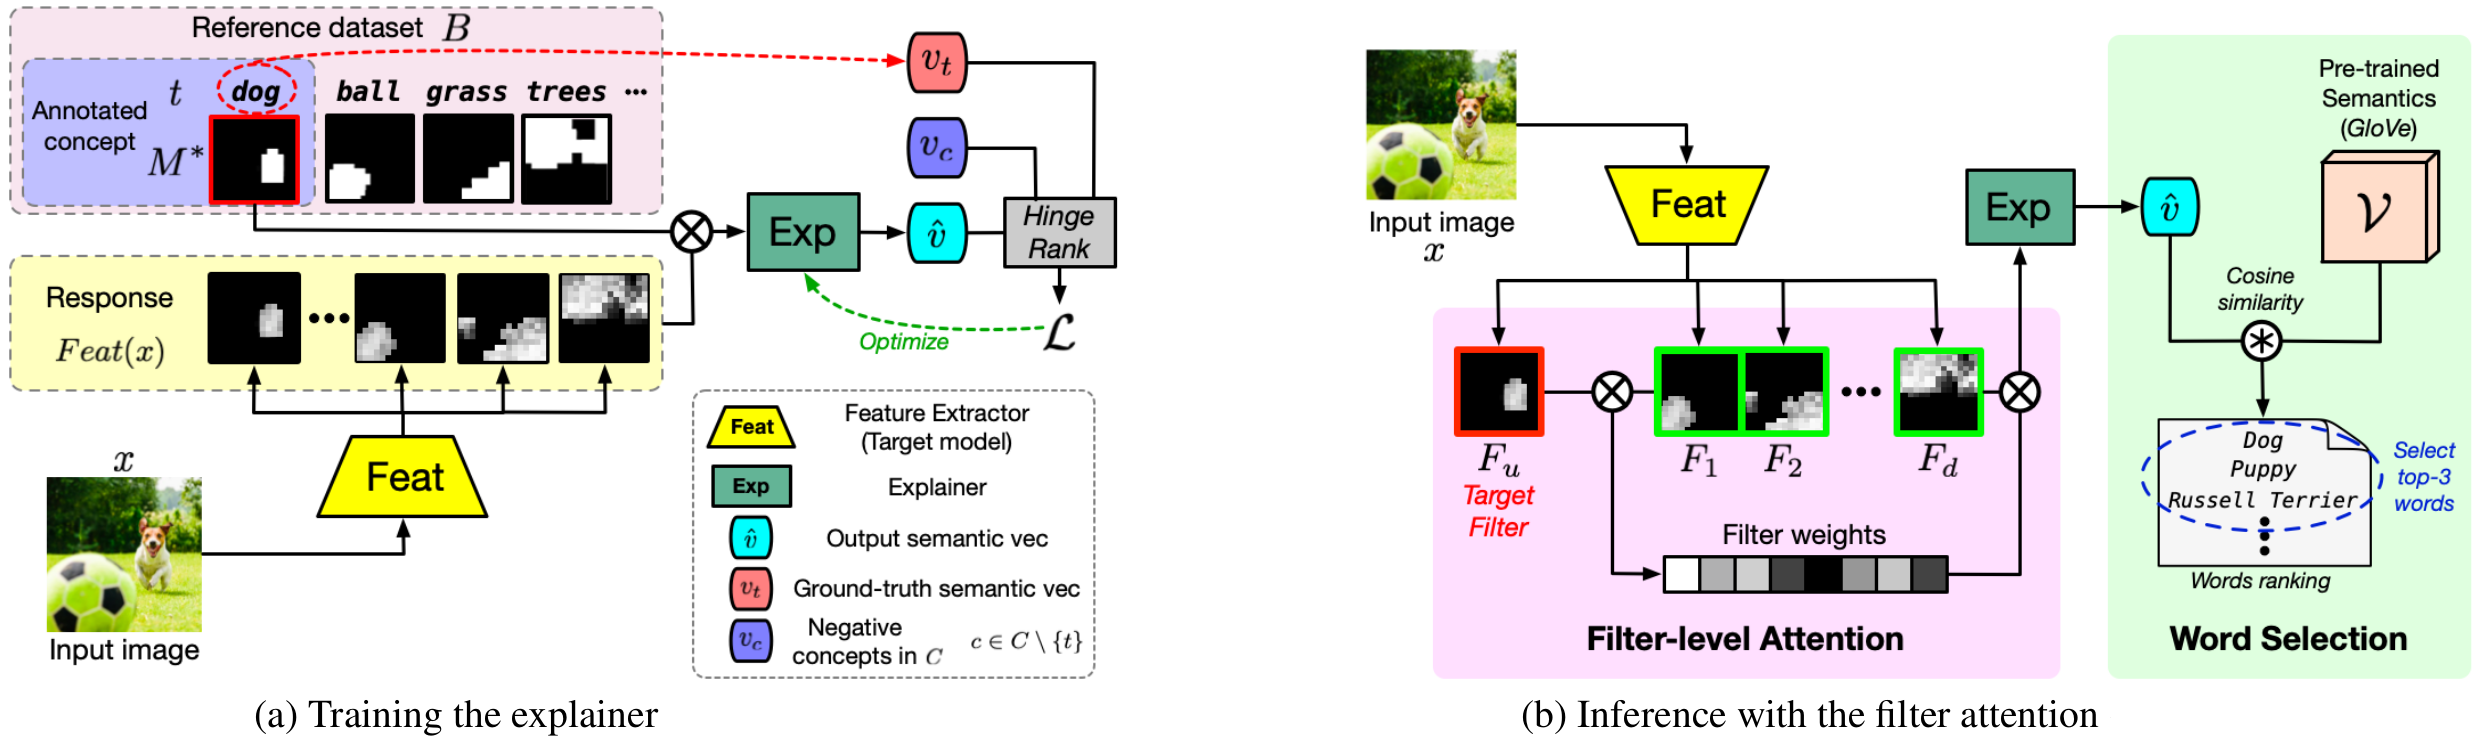
\includegraphics[width=\textwidth]{LaViSE_phases.png}
    \caption{Training and inference phase of the LaViSE framework \cite{yang2022explaining}.}
    \label{fig:LaViSE_phases}
\end{figure}

The LaViSE framework comprises two phases: a training phase and an inference phase, which can be seen in figure \ref{fig:LaViSE_phases}. During these phases, the framework uses two neural networks: a frozen \textit{feature extractor} $\Feat$, which consists of the first $L$ layers of any CNN that was pre-trained on an unknown dataset $D$, and a \textit{feature explainer} $\Exp$, which is a trainable 2-layer fully connected network (see section \ref{sec:Model descriptions}). Finally, GloVe embeddings \cite{pennington2014glove} are used to convert tokens to their semantic representations and vice versa.

\subsection{Training phase} \label{sec:Training phase}
The main issue of earlier work was that it required access to the original training data. LaViSE alleviates this by using a \textit{reference dataset} $B = \{(x_i, y_i)\}_{i=1}^n$ is used instead. Here, $x_i \in \mathbb{R}^{3 \times h \times w}$ is an input image and $y_i = \{(t_j, M_j)\}_{j=1}^k$ is a set of $k$ category labels $t_j$ with their corresponding segmentation masks $M_j \in \mathbb{R}^{h \times w}$. The set of all category labels in $B$ is given by $C$. During both inference and training, the first step is to use the extractor to transform an image and obtain its features with $F = \Feat(x) \in \mathbb{R}^{d \times h' \times w'}$. These features can be divided into $d$ \textit{filter activation maps} $[F_1, \dots, F_d]$, which have dimensionality $\mathbb{R}^{h' \times w'}$.
\\\\
Subsequently, the masked filter activation maps are multiplied elementwise with each mask. In turn, the result is passed through the explainer via $\hat v = \Exp(F \otimes M_j')$, which corresponds to the $\otimes$ symbol in figure \ref{fig:LaViSE_phases}a. If we define the semantic representation of the ground truth category to be $v_{t_j}$ and the set of all other categories to be $\{v_c \;|\; \forall c \in C,\; c \neq t_j\}$, we can formulate a variant of contrastive loss to train the explainer, which is given by
\begin{align*}
    \mathcal{L}(\theta) &= \sum_{j=1}^k \sum_{c \neq t_j} \max(0, 1 - \hat v \cdot v_{t_j} + \hat v \cdot v_c).
\end{align*}

\subsection{Inference phase} \label{sec:Inference phase}
During inference, we try to explain one target filter $F_u$ at a time. To do this, LaViSE uses a novel technique called \textit{filter-level attention}, which is visualized in figure \ref{fig:LaViSE_phases}b. In summary, the input to the explainer is $F^\text{att}$, which is defined with $F_k^\text{att} = a(F_u, F_k) \cdot F_k$ where $a$ represents the cosine similarity measure. The intuition behind this method is that important concepts are often implicitly represented and distributed over many filters. Lastly, after passing these features through the explainer, we search for the GloVe embedding closest to the model's prediction, establishing a mapping between the visual and semantic space.


\section{Methodology} \label{sec:Methodology}
% Explain your approach - did you use the author's code, or did you aim to re-implement the approach from the description in the paper? Summarize the resources (code, documentation, GPUs) that you used.
This section outlines which steps we undertook to replicate the experiments detailed in the original paper and how we resolved the ambiguity in the original paper. We focus on further reproducibility by describing our approach and design choices in detail.

\subsection{Model descriptions} \label{sec:Model descriptions}
% Include a description of each model or algorithm used. Be sure to list the type of model, the number of parameters, and other relevant info (e.g., if it is pre-trained).
We followed the paper's approach by conducting experiments with the PyTorch \cite{paszke2019pytorch} implementations of ResNet-18 (11.2M parameters) and ResNet-50 (25.6M parameters) \cite{he2016deep} as feature extractors. To test the generalizability of the method, we also trained the explainer with PyTorch's implementation of AlexNet \cite{krizhevsky2017imagenet} (62.4M parameters) as the feature extractor. All these models were pre-trained on ImageNet \cite{deng2009imagenet}.
\\\\
The feature explainer first squishes each filter activation map down to a single value using pooling layers used in the target CNN. This is followed by two linear layers separated by a ReLU activation function. In addition, batch normalization and dropout ($p=0.1$) are applied before each linear layer. Moreover, when there are $d$ filters, the feature explainer will have $d^2 + 303d + 900$ parameters.

\subsection{Reference datasets} \label{sec:Reference datasets}
% For each dataset, include 1) relevant statistics such as the number of examples and label distributions, 2) details of train/dev/test splits, 3) an explanation of any pre-processing done, and 4) a link to download the data (if available).
The original paper used two reference datasets: Common Objects in Context (COCO) \cite{coco} and Visual Genome (VG) \cite{krishna2017visual}. These datasets contain images with one or multiple \textit{annotations}, where each annotation contains an object label and its position in the image, given by a binary mask. Furthermore, COCO contains segmentation masks, while VG contains bounding boxes around objects. General statistics about these datasets are presented in table \ref{tab:datasets}. We adhered to the training/validation split used in the original paper to improve consistency in our experiments.

\begin{table}[b!]
    \centering
    \caption{\centering \textbf{Reference datasets.} The reference datasets used to train the feature explainer. The number of images and annotations are rounded to the nearest thousand.}
    \begin{tabular}{l r r r r r r r r r c c} \toprule
        \textbf{Dataset} & \multicolumn{3}{c}{\textbf{Images}} & \multicolumn{3}{c}{\textbf{Annotations}} & \multicolumn{3}{c}{\textbf{Categories}} & \textbf{URL} \\ \cmidrule(lr){2-4} \cmidrule(lr){5-7} \cmidrule(lr){8-10}
        & Train & Val & Total & Train & Val & Total & Train & Val & Total & & \\ \midrule
        COCO & 117k & 5k & 122k & 860k & 37k & 897k & 92 & 92 & 92 & \href{https://cocodataset.org/}{Link} \\
        VG & 90\% & 10\% & 93k & 90\% & 90\% & 1963k & 70\% & 30\% & 1128 & \href{http://visualgenome.org/}{Link} \\
    \bottomrule \end{tabular}
    \label{tab:datasets}
\end{table}

\subsubsection{Pre-processing} \label{sec:Pre-processing}
As in the original paper, pre-processing is performed exclusively on images in the VG dataset. In their paper, the authors describe that images without box-able annotations are removed, object categories are defined based on WordNet \cite{Fellbaum1998} synsets, and annotations of the same category in the same image are combined. Rare categories that appear fewer than 100 times are deleted. While we followed these pre-processing steps to the best of our ability, the results did not perfectly align. More specifically, the number of remaining images and categories we ended up with was around 12\% and 7\% lower than what was mentioned in the original paper. Further analysis revealed that our version was a subset of the original, which could be due to the order in which the pre-processing steps were applied; for example, our script removes images if they do not contain any annotations after the annotations with rare categories were removed. For exact replicability, we have made this pre-processing script available in our git repository\footnote{\url{https://github.com/ErikBuis/FACT2023}}.

\subsection{Experimental setup} \label{sec:Experimental setup}
% Include a description of how the experiments were set up that's clear enough a reader could replicate the setup.
% Include a description of the specific measure used to evaluate the experiments (e.g. accuracy, precision@K, BLEU score, etc.).
% Provide a link to your code.
All experiments were designed to assess at least one of the author's claims (introduced in section \ref{sec:Scope of reproducibility}).

\subsubsection{Claim 1: The proposed framework accurately maps the visual and semantic space using generic object detection datasets.}
To evaluate this claim, we replicated three original experiments as closely as possible. To be precise, we trained the explainer with ResNet-18 and ResNet-50 as the feature extractor, where VG was used as the reference dataset. However, for one of the experiments, we decided to use ImageNet for pre-training instead of COCO for three reasons. Firstly, training it ourselves was not feasible due to time and resource constraints. Secondly, using COCO as both a pre-training and reference dataset could lead to overfitting (as was also hypothesized by the original authors). Finally, pre-training all networks on ImageNet leads to a fairer comparison because only one variable (the reference dataset) is changed between experiments. For all these experiments, we followed the paper's approach in letting the explainer interpret each extractor's deepest filter layer, called \texttt{layer4} in both ResNet versions implemented in PyTorch.
In contrast, the number of epochs used to train the model was not given in the original paper. Realistically, we had limited resources, so we trained all models for exactly 30 epochs, where the model with the best validation loss was used during inference. By training for this long, we could still recognize trends in the data to assess the original work's reproducibility.

\subsubsection{Claim 2: The proposed framework can generate novel descriptions for learned filters beyond the categories defined in the reference dataset.}
To address this claim, we performed a qualitative analysis of the models trained on COCO. More specifically, we analyzed whether the model generated predictions that are not present in COCO and, if so, whether they are accurate. To accomplish this, we overlaid the activation heatmap over the corresponding input images. Next, we manually examined whether the model's novel predictions accurately described what the filters were focusing on.

\subsubsection{Claim 3: The proposed framework can analyze any trained CNN, regardless of whether or not the original training data is available.}
The original authors have limited their presentation of results to the ResNet architecture. To evaluate whether the LaViSE framework can generalize to work with other CNNs, we utilize AlexNet \cite{krizhevsky2017imagenet} as a feature extractor, as it is widely recognized as a prominent network in the deep learning field \cite{alom2018history}. We again trained a network to explain its deepest layer, which is called \texttt{features} in PyTorch.

\subsubsection{Evaluation measure} \label{sec:Evaluation measure}
The explainer models are evaluated using recall@$s$, which calculates the ratio of relevant results among a system's top $s$ outputs $W_{u, i}$. More precisely, we compute the recall@$s$ for each of the top $p$ images that activate a certain target filter $u$ the most and then average over the obtained scores. Here, we define the top $p$ images for filter $u$ to be $\{x_1^u, \dots, x_p^u\}$. Intuitively, we are looking for a fraction of ground-truth categories that the model predicted in a certain region of each image. To do this, we first find the region of activations $R_{u, i}$ that the model focuses on when looking at image $x_i^u$, which is a binary mask that indicates whether each activation is higher than the top 0.5\% of activations\footnote{This mask is overlaid with the original image to form the \textit{heatmap} shown in figure \ref{fig:ResNet-18-filter-output}.}. Mathematically, $R_{u, i} = [\Feat(x_i^u) > T_u]$, where $p(\Feat(x_i) > T_u) > 0.005$. Furthermore, since we are using the validation set, we can access $k$ annotations corresponding to the image. These can be used to calculate the ground-truth concepts to compare to, which are given by $G_{u, i} = \{t_j \;|\; \forall_{1 \leq j \leq k},\; \text{IoU}(M_j, R_{u, i}) > 0.04\}$, where $\text{IoU}$ calculates the intersection-over-union score between its arguments. Finally, we can calculate the recall as follows:
\begin{align*}
    \text{Recall@}s_{u, i} = \frac{| W_{u, i} \cap G_{u, i} |}{| G_{u, i} |}.
\end{align*}

\subsection{Hyperparameters} \label{sec:Hyperparameters}
% Describe how the hyperparameter values were set. If there was a hyperparameter search done, be sure to include the range of hyperparameters searched over, the method used to search (e.g. manual search, random search, Bayesian optimization, etc.), and the best hyperparameters found. Include the number of total experiments (e.g. hyperparameter trials). You can also include all results from that search (not just the best-found results).
Due to the learning rate used in the original experiments being unknown, we employed the \texttt{DAdaptAdam} optimizer \cite{defazio2023learning}, which utilizes a dynamic adaptation technique for the learning rate, eliminating the need for manual tuning. Additionally, we selected the maximum batch size that could fit in the GPU (2048 samples per batch).

\subsection{Improving the codebase} \label{sec:Improving the codebase}
In order to reproduce the experiments described in the original paper, we obtained the authors' PyTorch implementation from their public repository on GitHub \cite{lavise-repo}. However, the code lacked completeness, efficiency, and documentation. Therefore, the first step was to ensure the code was functional by adding missing code and debugging where necessary.
\\\\
Most prominently, we created functions for calculating the recall measure, plotting activation heatmaps, and pre-processing and loading the VG dataset. Next, we added docstrings and type hints to all functions to improve code readability and catch potential errors. We added the functionality for using a fixed seed, added scripts to download and pre-process both datasets automatically, and made the coding style consistent. In doing this, we aimed to facilitate future maintainability and reproducibility.
\\\\
Lastly, we improved the code's efficiency to save on required computational resources. More specifically, this was accomplished by creating a faster algorithm for finding the $p$ images that activate certain filters the most, memoizing the results of expensive function calls, decreasing the number of I/O calls to speed up data loading, moving operations from the CPU to the GPU, and parallelizing sequential operations. Especially the inference code underwent extensive re-engineering to achieve substantial performance improvements, resulting in a speedup of 12x.

\subsection{Computational requirements} \label{sec:Computational requirements}
% Include a description of the hardware used, such as the GPU or CPU the experiments were run on.
% For each model, include a measure of the average runtime (e.g. average time to predict labels for a given validation set with a particular batch size).
% For each experiment, include the total computational requirements (e.g. the total GPU hours spent).
% (Note: you'll likely have to record this as you run your experiments, so it's better to think about it ahead of time). Generally, consider the perspective of a reader who wants to use the approach described in the paper --- list what they would find useful.
Information about neither the hardware used nor the GPU hours required to perform the experiments was given in the original work. Consequently, we chose the fastest option available to us to perform our experiments: an Nvidia A100 GPU with 40 GB of RAM running on a Google Cloud Platform (GCP) computing instance. Training each model cost 15 hours on average, and to compute the heatmaps and recall score, 30 extra minutes were required. In the end, the total hours spent to obtain all results presented in this report amounted to 62 GPU hours.


\section{Results} \label{sec:Results}
% Start with a high-level overview of your results. Do your results support the main claims of the original paper? Keep this section as factual and precise as possible, reserve your judgement and discussion points for the next "Discussion" section.
\begin{table}[t!]
    \centering
    \caption{\centering \textbf{Results reproducing original paper.} Recall (R@$s$) scores of the original paper versus ours.}
    \begin{tabular}{c c c c c c c} \toprule
        \multicolumn{1}{c}{\textbf{\begin{tabular}[c]{@{}c@{}} Model \\ \& Layer \end{tabular}}} &
        \multicolumn{1}{c}{\textbf{Implementation}} &
        \multicolumn{1}{c}{\textbf{\begin{tabular}[c]{@{}c@{}} Original \\ dataset \end{tabular}}} &
        \multicolumn{1}{c}{\textbf{\begin{tabular}[c]{@{}c@{}} Reference \\ dataset \end{tabular}}} &
        \multicolumn{1}{c}{\textbf{R@5}} &
        \multicolumn{1}{c}{\textbf{R@10}} &
        \multicolumn{1}{c}{\textbf{R@20}} \\ \midrule

        \begin{tabular}[c]{@{}c@{}} ResNet-18 \\ \texttt{layer4} \end{tabular} &
        \begin{tabular}[c]{@{}c@{}} Original \\ Ours \end{tabular} &
        \begin{tabular}[c]{@{}c@{}} COCO \\ ImageNet \end{tabular} &
        \begin{tabular}[c]{@{}c@{}} COCO \\ COCO \end{tabular} &
        \begin{tabular}[c]{@{}c@{}} 0.675 \\ 0.448 \end{tabular} &
        \begin{tabular}[c]{@{}c@{}} 0.728 \\ 0.477 \end{tabular} &
        \begin{tabular}[c]{@{}c@{}} 0.776 \\ 0.497 \end{tabular} \\ \midrule

        \begin{tabular}[c]{@{}c@{}} ResNet-18 \\ \texttt{layer4} \end{tabular} &
        \begin{tabular}[c]{@{}c@{}} Original \\ Ours \end{tabular} &
        \begin{tabular}[c]{@{}c@{}} ImageNet \\ ImageNet \end{tabular} &
        \begin{tabular}[c]{@{}c@{}} VG \\ VG \end{tabular} &
        \begin{tabular}[c]{@{}c@{}} 0.273 \\ 0.163 \end{tabular} &
        \begin{tabular}[c]{@{}c@{}} 0.353 \\ 0.198 \end{tabular} &
        \begin{tabular}[c]{@{}c@{}} 0.429 \\ 0.243 \end{tabular} \\ \midrule

        \begin{tabular}[c]{@{}c@{}} ResNet-50 \\ \texttt{layer4} \end{tabular} &
        \begin{tabular}[c]{@{}c@{}} Original \\ Ours \end{tabular} &
        \begin{tabular}[c]{@{}c@{}} ImageNet \\ ImageNet \end{tabular} &
        \begin{tabular}[c]{@{}c@{}} VG \\ VG \end{tabular} &
        \begin{tabular}[c]{@{}c@{}} 0.226 \\ 0.132 \end{tabular} &
        \begin{tabular}[c]{@{}c@{}} 0.302 \\ 0.164 \end{tabular} &
        \begin{tabular}[c]{@{}c@{}} 0.373 \\ 0.197 \end{tabular} \\
    \bottomrule \end{tabular}
    \label{tab:Results reproducing original paper}
\end{table}

Table \ref{tab:Results reproducing original paper} presents our quantitative results, comparing them to the original paper's results. The subsequent sections will assess the validity of the authors' claims when considering these results.

\subsection{Results reproducing original paper} \label{sec:Results reproducing original paper}
% For each experiment, say 1) which claim in Section \ref{sec:Scope of reproducibility} it supports, and 2) if it successfully reproduced the associated experiment in the original paper.
% For example, an experiment training and evaluating a model on a dataset may support a claim that that model outperforms some baseline.
% Logically group related results into sections.

\subsubsection{Claim 1: The proposed framework accurately maps the visual and semantic space using generic object detection datasets.}
Table \ref{tab:Results reproducing original paper} presents our experiment outcomes and a comparison with the authors' results. While the original work recorded considerably better recall scores on all experiments, we can still see that the main trends are comparable. The rationale behind this is that the recall scores we get are still sufficient to support the claim: for example, the recall@5 score of ResNet-50, which is only 0.132, can intuitively be interpreted as the model predicting the correct category out of VG's 1128 categories around 13.2\% of the time. Adding to this, most of our trained models reached their highest validation loss after the last training epoch, indicating that improvements were still being made. Moreover, figure \ref{fig:ResNet-18-filter-output}, which displays some examples of the explainer's predictions, shows that the framework predicts primarily meaningful and relevant words for the masked objects in the images.

\subsubsection{Claim 2: The proposed framework can generate novel descriptions for learned filters beyond the categories defined in the reference dataset.}
This claim is validated by figure \ref{fig:ResNet-18-filter-output}, which illustrates that the model accurately predicts words (shown in green) that are not present in the reference dataset but accurately describes the filters. Remarkably, the filters mostly predict out-of-dataset words, which suggests that the model's capabilities are very generalizable. However, this may be caused by the predictions being morphological variants of words contained in the dataset, which could be an interesting area for future research. Finally, LaViSE can accurately generate multiple semantic categories when explaining some filters that focus on more than one category.

\begin{figure}[hb!]
    \centering
    \includegraphics[width=0.6\textwidth]{ResNet-18-filter-output.png}
    \caption{Visualization of explainer predictions when interpreting filters 150, 275 and 400 in \texttt{layer4} of ResNet-18, with COCO as the reference dataset.}
    \label{fig:ResNet-18-filter-output}
\end{figure}

\subsection{Results beyond original paper} \label{sec:Results beyond original paper}
% Often papers don't include enough information to fully specify their experiments, so some additional experimentation may be necessary. For example, it might be the case that batch size was not specified, and so different batch sizes need to be evaluated to reproduce the original results. Include the results of any additional experiments here. Note: this won't be necessary for all reproductions.

\subsubsection{Claim 3: The proposed framework can analyze any trained CNN, regardless of whether or not the original training data is available.}
To assess the validity of this claim, we have tested LaViSE's applicability to AlexNet. Table \ref{tab:Results beyond original paper} presents these results quantitatively. Our implementation achieved recall scores comparable to ResNet-18 trained with COCO (shown in table \ref{tab:Results reproducing original paper}), confirming the claim's validity.

\begin{table}[t!]
    \centering
    \caption{\centering \textbf{Results beyond original paper.} Recall (R@$s$) score of an additional experiment to assess the generalizability of the method.}
    \begin{tabular}{c c c c c c} \toprule
        \multicolumn{1}{c}{\textbf{\begin{tabular}[c]{@{}c@{}} Model \\ \& Layer \end{tabular}}} &
        \multicolumn{1}{c}{\textbf{\begin{tabular}[c]{@{}c@{}} Original \\ dataset \end{tabular}}} &
        \multicolumn{1}{c}{\textbf{\begin{tabular}[c]{@{}c@{}} Reference \\ dataset \end{tabular}}} &
        \multicolumn{1}{c}{\textbf{R@5}} &
        \multicolumn{1}{c}{\textbf{R@10}} &
        \multicolumn{1}{c}{\textbf{R@20}} \\ \midrule

        \begin{tabular}[c]{@{}c@{}} AlexNet \\ \texttt{features} \end{tabular} & ImageNet & COCO & 0.551 & 0.571 & 0.600 \\
    \bottomrule \end{tabular}
    \label{tab:Results beyond original paper}
\end{table}


\section{Discussion} \label{sec:Discussion}
% Give your judgement on if your experimental results support the claims of the paper. Discuss the strengths and weaknesses of your approach - perhaps you didn't have time to run all the experiments, or perhaps you did additional experiments that further strengthened the claims in the paper.
Our results show that the LaViSE framework effectively maps the visual and semantic space, as demonstrated by the recall scores recorded on both ResNet models and our additional test on AlexNet, where LaViSE achieved a comparable score. This supports the first and third claims of the authors (see section \ref{sec:Results reproducing original paper}). Additionally, our results confirm that LaViSE can generate novel descriptions for latent representations of filters: the explainer accurately predicts words that are not present in the reference dataset (see section \ref{sec:Results beyond original paper}).
\\\\
Despite this, the author's recall scores were consistently higher. The most important reason for this was that it was challenging to reproduce the authors' results accurately due to the absence of crucial information regarding the implementation, which was discussed more thoroughly in section \ref{sec:Improving the codebase}. Moreover, as discussed in section \ref{sec:Pre-processing}, slightly different pre-processing methods may have affected the training procedure and, in turn, the final results. Furthermore, the number of epochs to train for may have been much higher, which would severely limit the model's ability to perform rigorously.
\\\\
Even though our results aligned with the author's claims, there are still some limitations and potential areas for improvement. Further experiments could be conducted on a broader range of CNN architectures to evaluate the generalizability of LaViSE to a fuller extent, as our research was limited to AlexNet and ResNet.
\\\\
In conclusion, our results support the claims made in the original paper and show that LaViSE is a reliable and effective tool for mapping the visual space to the semantic space. However, more research could be conducted to assess its capabilities more precisely and to find its strengths and weaknesses.

\subsection{What was easy} \label{sec:What was easy}
% Give your judgement of what was easy to reproduce. Perhaps the author's code is clearly written and easy to run, so it was easy to verify the majority of original claims. Or, the explanation in the paper was really easy to follow and put into code.
% Be careful not to give sweeping generalizations. Something that is easy for you might be difficult to others. Put what was easy in context and explain why it was easy (e.g. code had extensive API documentation and a lot of examples that matched experiments in papers).
We particularly appreciated the paper's easily comprehensible writing style, which made it easy to understand. The use of figures, particularly those illustrating the phases of the LaViSE framework, was helpful in providing a clear and concise overview of the training and inference processes, which helped us in our implementation.

\subsection{What was difficult} \label{sec:What was difficult}
The implementation of the methodology outlined in this paper presented challenges, primarily due to the limited documentation and insufficient details regarding parts that were not included in the existing codebase. This made it challenging to comprehend the existing code's functioning and pinpoint the bugs' origin. Furthermore, the bugs impeded the implementation process by causing unforeseen errors and crashes, complicating the determination of whether the issues arose from implementing the new method or were intrinsic to the existing codebase. Lastly, it was only feasible to recreate some experiments; in particular, the experiments that required an extractor to be pre-trained would take significant time and resources to verify.

\subsection{Communication with original authors} \label{sec:Communication with original authors}
We sought assistance from the original authors to clarify missing information and aspects that needed to be fixed as expected. Unfortunately, they informed us that they were occupied with other commitments. Nevertheless, we still sought further understanding of the repository and respectfully requested information regarding its completeness, the settings employed for training, and the pre-trained weights on the COCO dataset. Alas, we did not receive any further response.
